\documentclass[a4paper, 12pt]{article}

\usepackage{amsmath}
\usepackage{graphicx}
\begin{document}
\pagenumbering{gobble}
\title{\textbf{Project Report on: \\ STUDY ON DYNAMIC ROBOT PATH PLANNING}}
\date{$26^{th}$ November, 2017}

\maketitle
\centerline{}
\centerline{}
\centerline{\textit{\large Study Project Report}}
\centerline{}
\centerline{}
\centerline{}
\centerline{\textit{\large Under the guidance of}}
\centerline{}
\centerline{\newline Dr. Surekha Bhanot}
\centerline{Professor}
\centerline{BITS Pilani}
\vfill
\rightline{Submitted By:}
\rightline{}
\rightline{Arjun Gupta}
\rightline{Msc. (Hons) Mathematics and B.E. EEE 4th year student} 
\rightline{2014B4A30754P}
\rightline{BITS Pilani, Pilani Campus}
\rightline{}
\rightline{}
\rightline{Rasal Kumar}
\rightline{Msc. (Hons) Mathematics and B.E. ENI 4th year student}
\rightline{2014B4A80801P}
\rightline{BITS Pilani, Pilani Campus}

\newpage
\section*{Acknowledgment}
\addcontentsline{toc}{section}{Acknowledgment}

We would like to express my gratitude to my project in-charge Dr. Surekha Bhanot. We were quite eager to learn about Dynamic Path Planning and we are extremely grateful for the opportunity provided to us to work under her guidance on the topic. Her constant guidance, insights and regular discussions have been extremely valuable. She has provided us with a wonderful research experience, which has shaped our approach to tackle research problems especially on path planning. We will be eternally grateful for the guidance provided.

\newpage
\tableofcontents
\newpage
%\section*{Abstract}
%\addcontentsline{toc}{section}{Abstract}


\newpage
\pagenumbering{arabic}

\section{Introduction}
In most cases such as factory warehouse, mobile robots are required to navigate from starting point to the destination without collision according to some criterion. The need for finding the shortest routine through known obstacles leads to a globally optimal path planning problem. Path planning is considered as a major problem in robotics since its complexity increases exponentially with the dimensions of the configuration space. The configuration space is defined as the space that the physical system may attain with respect to the external and environmental constraints. In recent years many intelligent algorithms have been developed for path planning of mobile robot, such as artificial neural networks,genetic algorithms and ant colony optimization(ACO). ACO algorithms has prominent advantages, such as positive feedback search mechanism, distributed computation and has better probability in achieving globally optimal solution. \\
\\
In this study, we propose a model which uses a neural network (NN) trained by backpropagation algorithm\cite{refer2} to move along a path obtained by ACO. The NN gives the output as heading angle form the data as received by the ultrasonic sensors, thus preventing the bot from any collision. A suitable algorithm is proposed to interpret the data received by the sensors and then finally move along the obtained optimum path. Free space model of mobile robot is established by using visible graph method and ACO algorithm is utilized in this model to search a global collision free path which is the shortest routine through known static obstacles. Results of simulation experiments are shared in the report and are discussed in detail.\\
\\ 
The report is structured as; section 2 discusses the ACO algorithm briefly and the MATLAB results obtained to support the theory. In section 3 a brief introduction of Neural Network and later Backpropagation algorithm is given. In section 4 we have discussed our model and the results obtained. Finally we conclude in section 5 and propose the future expectations.

\section{Any Colony Optimization}
The Ant Colony Optimization algorithm (ACO) is a probabilistic technique for solving computational problems which can be reduced to finding good paths through graphs \cite{refer1}. Ant colony optimization (ACO) takes inspiration from the foraging behavior of some ant species. These ants deposit pheromone on the ground in order to mark some favorable path that should be followed by other members of the colony. Ant colony optimization exploits a similar mechanism for solving optimization problems. Various experiments have found that the in the long run colony of ants converge to the shortest possible path thus resulting in global optimum path. In our model we aim to find the global optimum path by using ACO if possible. Initially to understand the basic behavior of ant colony we used MATLAB as a platform to obtain results. We built to track following the curve equations: 1. $y_1 = x$ and 2. $y_2 = x^2$. The probability of the decision taken by the ant is determined by the formula:
\begin{equation}
Probability = \frac{t_s + \phi(1,1)^2}{(t_s + \phi(1,1)^2)+(t_s + \phi(1,2)^2)}
\end{equation}
where $t_s$ is the time taken along the shortest path, $\phi(1,1)$ denotes the pheromone level on the shortest path and $\phi(1,2)$ denotes pheromone level on the longer path. In our code we have taken 10 ants and the screenshots of some part of the result obtained show in fig \ref{fig1}. 
\begin{figure}[!h]
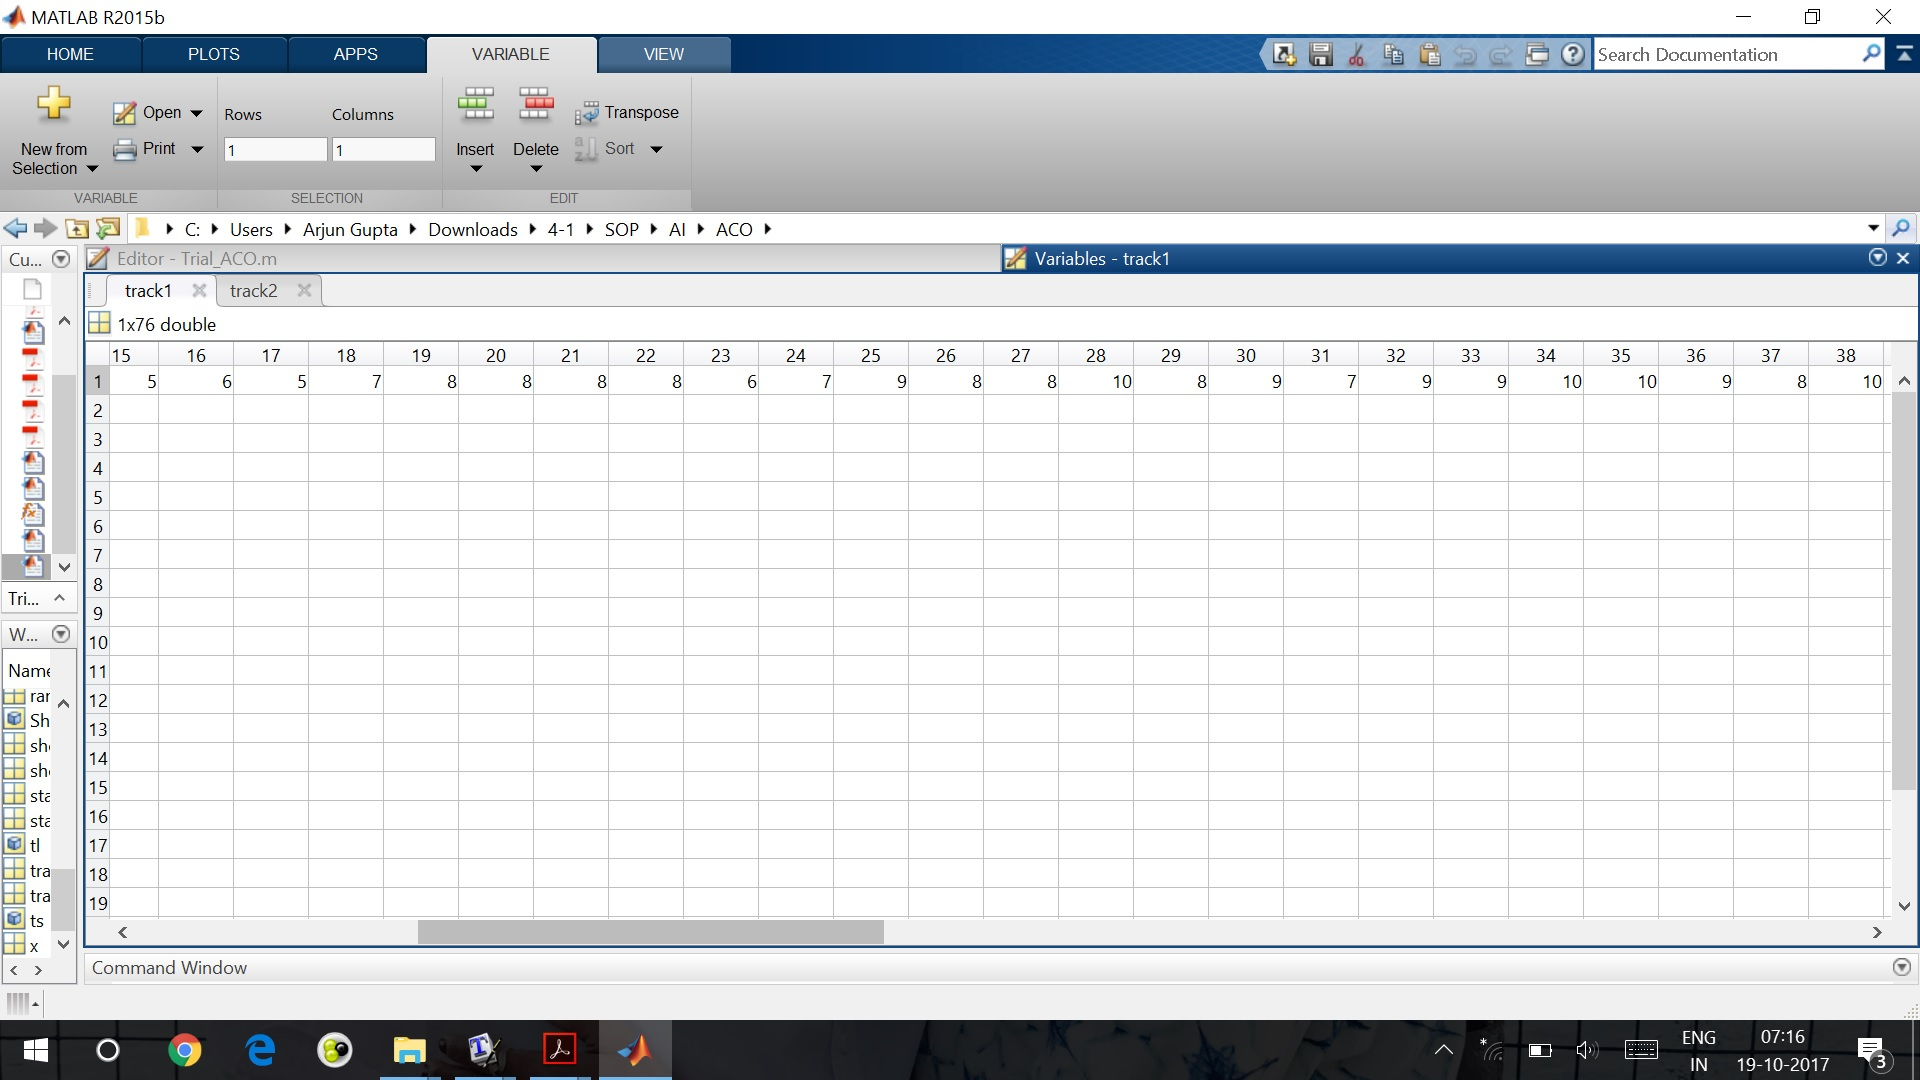
\includegraphics[height = 2 in, width= \linewidth]{ACO_track1.png}

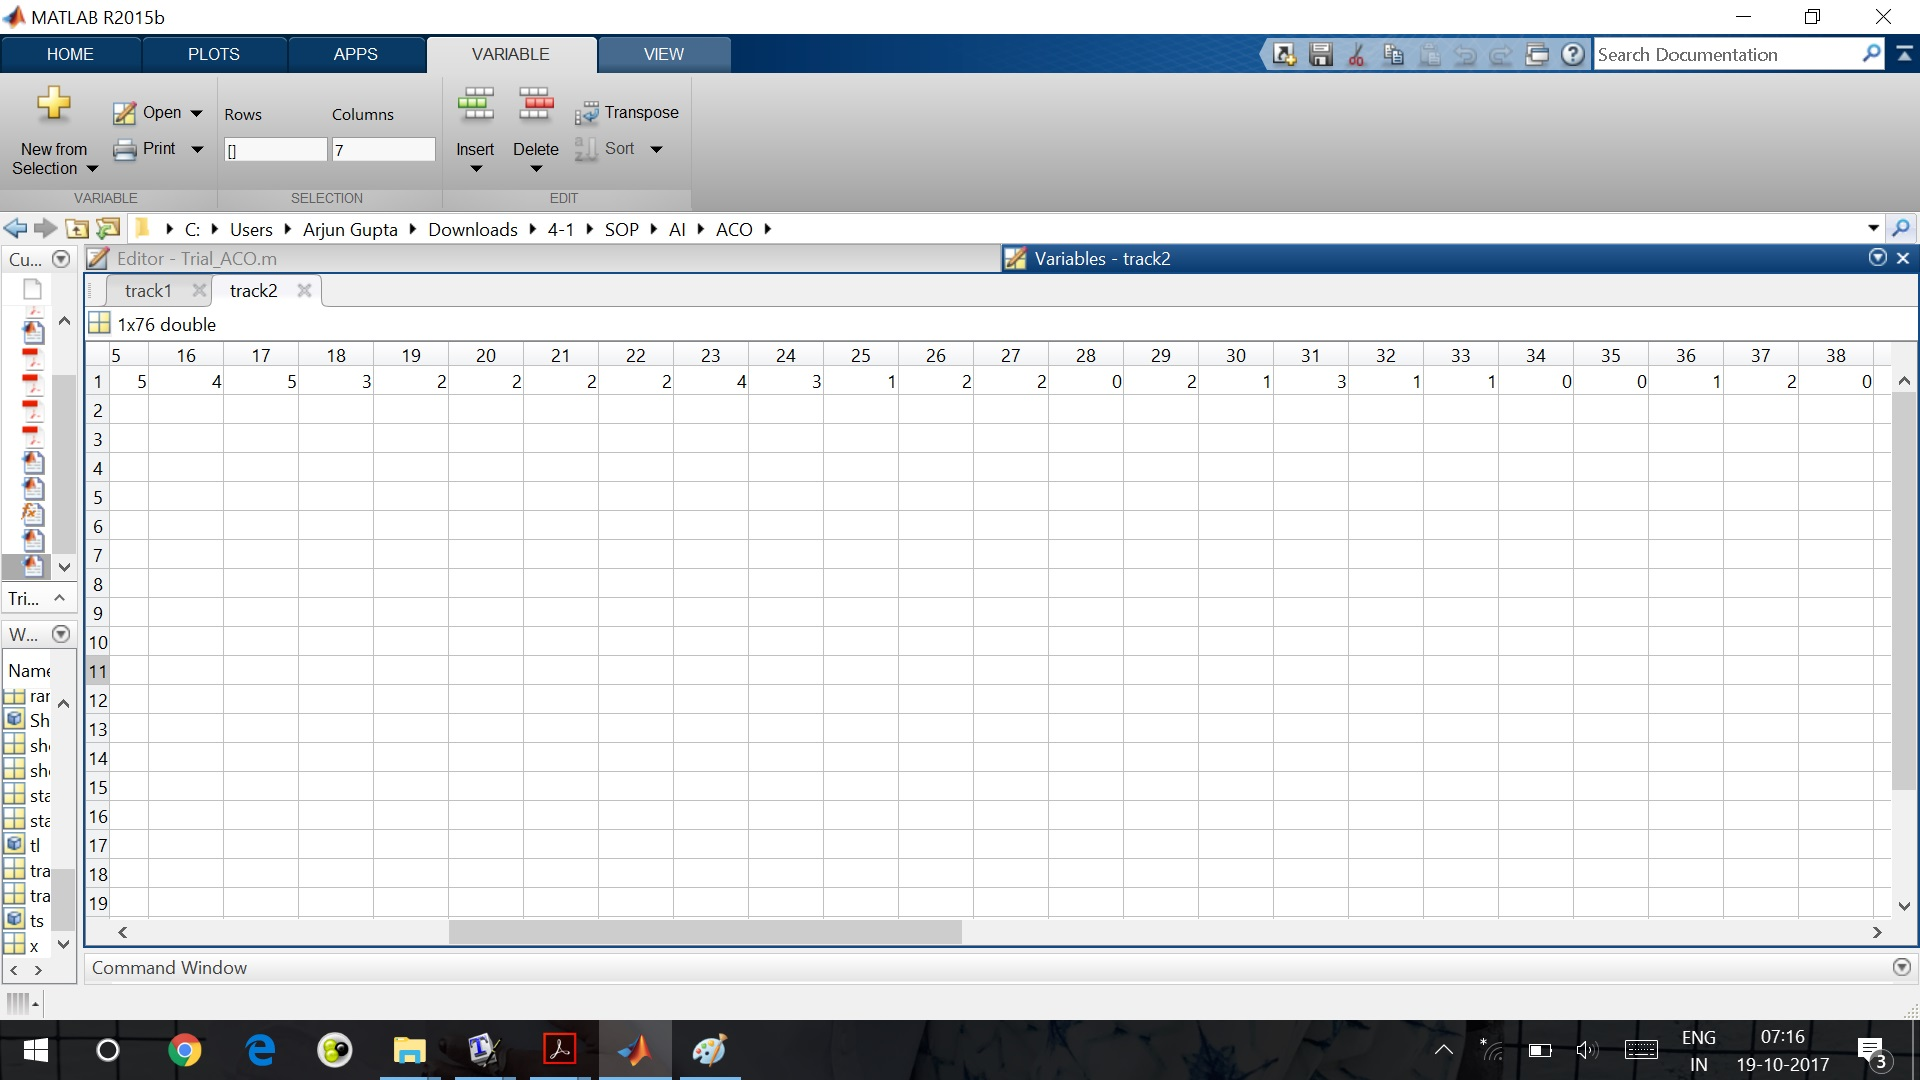
\includegraphics[height = 2 in, width= \linewidth]{ACO_track2.png}
\caption{Number of ants traveling on track 1 and  track 2 in different iterations}
\label{fig1}
\end{figure}
The result obtain verifies the the theoretical assertions claimed by the several studies. 

\section{Artificial Neural Network}
Artificial Neural Network (ANN) is an efficient computing system whose central theme is borrowed from the analogy of biological neural networks. ANNs are also named as “artificial neural systems,” or “parallel distributed processing systems,” or “connectionist systems.” ANN acquires a large collection of units that are interconnected in some pattern to allow communication between the units. These units, also referred to as nodes or neurons, are simple processors which operate in parallel. Every neuron is connected with other neuron through a connection link. Each connection link is associated with a weight that has information about the input signal. This is the most useful information for neurons to solve a particular problem because the weight usually excites or inhibits the signal that is being communicated. Each neuron has an internal state, which is called an activation signal. Output signals, which are produced after combining the input signals and activation rule, may be sent to other units. As per the network topology the ANN can be classified as:
\begin{enumerate}
\item Feedforward Network: A feedforward neural network is an artificial neural network wherein connections between the units do not form a cycle.The feedforward neural network was the first and simplest type of artificial neural network devised. In this network, the information moves in only one direction, forward, from the input nodes, through the hidden nodes (if any) and to the output nodes. There are no cycles or loops in the network. It is of two types: 
\begin{enumerate}
\item Single layer feedforward network: The simplest kind of neural network is a single-layer perceptron network, which consists of a single layer of output nodes; the inputs are fed directly to the outputs via a series of weights. In this way it can be considered the simplest kind of feed-forward network. The sum of the products of the weights and the inputs is calculated in each node, and if the value is above some threshold (typically 0) the neuron fires and takes the activated value (typically 1); otherwise it takes the deactivated value (typically -1). Neurons with this kind of activation function are also called artificial neurons or linear threshold units. In the literature the term perceptron often refers to networks consisting of just one of these units.A perceptron can be created using any values for the activated and deactivated states as long as the threshold value lies between the two.Perceptrons can be trained by a simple learning algorithm that is usually called the delta rule. It calculates the errors between calculated output and sample output data, and uses this to create an adjustment to the weights, thus implementing a form of gradient descent.
\item Multilayer feedforward network: This class of networks consists of multiple layers of computational units, usually interconnected in a feed-forward way. Each neuron in one layer has directed connections to the neurons of the subsequent layer. In many applications the units of these networks apply a sigmoid function as an activation function. Multi-layer networks use a variety of learning techniques, the most popular being back-propagation. Here, the output values are compared with the correct answer to compute the value of some predefined error-function. By various techniques, the error is then fed back through the network. Using this information, the algorithm adjusts the weights of each connection in order to reduce the value of the error function by some small amount. After repeating this process for a sufficiently large number of training cycles, the network will usually converge to some state where the error of the calculations is small. In this case, one would say that the network has learned a certain target function. To adjust weights properly, one applies a general method for non-linear optimization that is called gradient descent. For this, the network calculates the derivative of the error function with respect to the network weights, and changes the weights such that the error decreases (thus going downhill on the surface of the error function). For this reason, back-propagation can only be applied on networks with differentiable activation functions.
\end{enumerate}
\item Feedback Network
\begin{enumerate}
\item Recurrent Networks: A recurrent neural network (RNN) is a class of artificial neural network where connections between units form a directed cycle. This allows it to exhibit dynamic temporal behavior. Unlike feedforward neural networks, RNNs can use their internal memory to process arbitrary sequences of inputs.
\item Fully Recurrent Networks: Basic RNNs are a network of neuron-like nodes, each with a directed (one-way) connection to every other node.[citation needed] Each node (neuron) has a time-varying real-valued activation. Each connection (synapse) has a modifiable real-valued weight. Nodes are either input nodes (receiving data from outside the network), output nodes (yielding results), or hidden nodes (that modify the data en route from input to output).

For supervised learning in discrete time settings, sequences of real-valued input vectors arrive at the input nodes, one vector at a time. At any given time step, each non-input unit computes its current activation (result) as a nonlinear function of the weighted sum of the activations of all units that connect to it. Supervisor-given target activations can be supplied for some output units at certain time steps. For example, if the input sequence is a speech signal corresponding to a spoken digit, the final target output at the end of the sequence may be a label classifying the digit.

In reinforcement learning settings, no teacher provides target signals. Instead a fitness function or reward function is occasionally used to evaluate the RNN's performance, which influences its input stream through output units connected to actuators that affect the environment. This might be used to play a game in which progress is measured with the number of points won.
\item Elman and Jordan Network: An Elman network is a three-layer network (arranged horizontally as x, y, and z in the illustration) with the addition of a set of "context units" (u in the illustration). The middle (hidden) layer is connected to these context units fixed with a weight of one. At each time step, the input is fed-forward and a learning rule is applied. The fixed back-connections save a copy of the previous values of the hidden units in the context units (since they propagate over the connections before the learning rule is applied). Thus the network can maintain a sort of state, allowing it to perform such tasks as sequence-prediction that are beyond the power of a standard multilayer perceptron.

Jordan networks are similar to Elman networks. The context units are fed from the output layer instead of the hidden layer. The context units in a Jordan network are also referred to as the state layer. They have a recurrent connection to themselves.

\end{enumerate}
\end{enumerate}
 
\subsection{Back Propagation NN}
Back Propagation Neural Network (BPNN) is a multi layer neural network consisting of the input layer, at least one hidden layer and output layer. As its name suggests, back propagation will take place in this network. The error which is calculated at the output layer, by comparing the target output and the actual output, will be propagated back towards the input layer. The architecture of back propagation network is shown below in fig \ref{fig2}. As shown in the diagram, the architecture of BPN has three interconnected layers having weights on them. The hidden layer as well as the output layer also has bias, whose weight is always 1, on them. As is clear from the diagram, the working of BPN is in two phases. One phase sends the signal from the input layer to the output layer, and the other phase back propagates the error from the output layer to the input layer. 
\begin{figure}[!h]
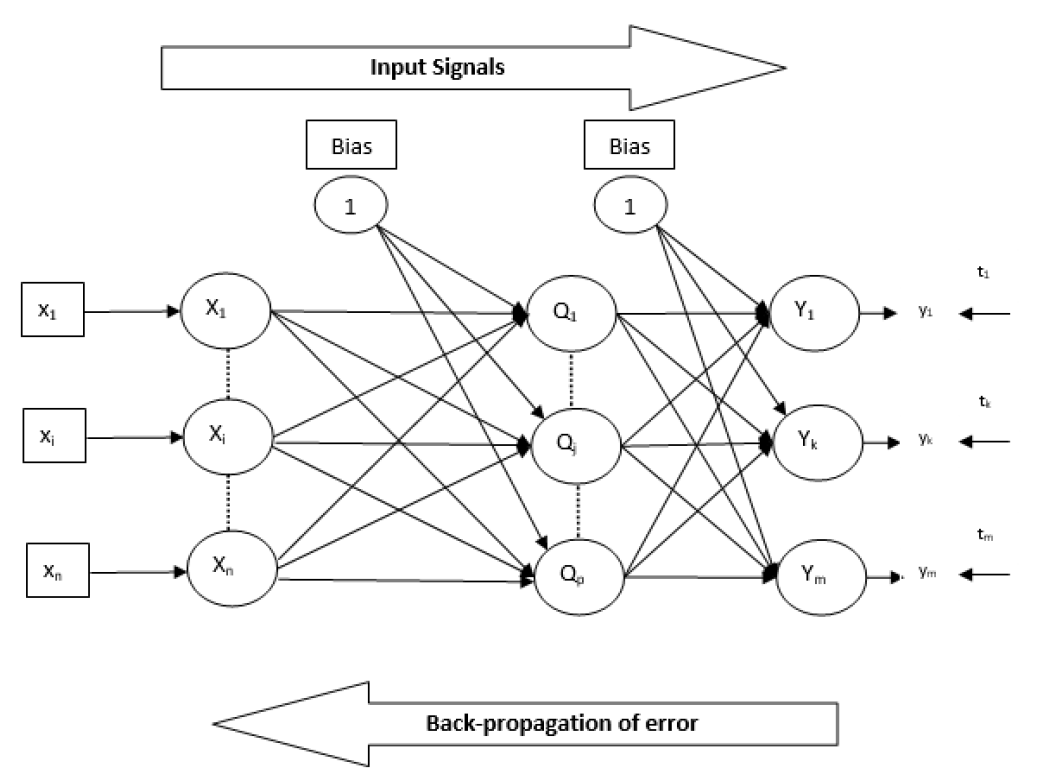
\includegraphics[height =2 in, width = \linewidth]{Architecture.png}
\caption{Architecture of BPNN}
\label{fig2}
\end{figure}

\section{Dynamic Vehicle Model}
Vehicle stability control systems that prevent vehicles from spinning and
drifting out have been developed and recently commercialized by several
automotive manufacturers. Such stability control systems are also often
referred to as yaw control systems or electronic stability control systems.
Figure below schematically shows the function of a yaw control system.
In this figure, the lower curve shows the trajectory that the vehicle would
follow in response to a steering input from the driver if the road were dry
and had a high tire-road friction coefficient. In this case the high friction
coefficient is able to provide the lateral force required by the vehicle to
negotiate the curved road. If the coefficient of friction were small or if the vehicle speed were too high, then the vehicle would be unable to follow
the nominal motion required by the driver – it would instead travel on a
trajectory of larger radius (smaller curvature), as shown in the upper curve of Figure below. The function of the yaw control system is to restore the yaw
velocity of the vehicle as much as possible to the nominal motion expected
by the driver. If the friction coefficient is very small, it might not be possible to entirely achieve the nominal yaw rate motion that would be achieved by the driver on a high friction coefficient road surface. In this case, the yaw control system would partially succeed by making the vehicle’s yaw rate closer to the expected nominal yaw rate.
Many companies have investigated and developed yaw control systems
during the last ten years through simulations and on prototype experimental
vehicles. Some of these yaw control systems have also been commercialized
on production vehicles.
Three types of stability control systems have been proposed and developed
for yaw control:
Differential Braking systems which utilize the ABS brake system on the
vehicle to apply differential braking between the right and left wheels to
control yaw moment.
Steer-by-Wire systems which modify the driver’s steering angle input
and add a correction steering angle to the wheels
20 Chapter 2
Active Torque Distribution systems which utilize active differentials
and all wheel drive technology to independently control the drive torque
distributed to each wheel and thus provide active control of both traction and yaw moment.
\section{Artificial Neural Network as a Controller}
Artificial Neural Network “ANN” has been applied successfully to a wide range of control system applications in recent years. Artificial neural networks have high learning and nonlinear mapping essences and its parallel and distributed structure can provide a nonlinear mapping between inputs and outputs of an electric drive system, without the knowledge of any predetermined model. This makes ANN a good choice to be used in the adaptation mechanism of a MRAC system.
\section{Proposed Model and Results}
In our model we have trained our neural network using back propagation algorithm. The data is obtained from the thesis report of Rohan Kumar Sabat and Anshu J Behera of NIT Rourkela. Training of neural network is done using the parameter values as shown in the fig \ref{fig3}. Number of layers for the neural network is obtained by using different number of layers and then choosing the one with optimum result. The structure of our neural network is shown in fig \ref{fig4}. The training process interim screenshot is shown in fig \ref{fig5}. The result obtained after training the neural net on the chosen data set, the results obtained are shown in fig \ref{fig6}. The data contains 4 columns where first three contain the lateral left, right and front distance of vehicle from the obstacles. These three inputs are gives as the input and the fourth column contains the heading angle which is set as the target data for the model. We obtain the the three lateral distances using sensors and the NN outputs the heading angle. We used the same data we used for training to find the trajectory of the bot. The result obtained is shown in fig \ref{fig7}.
\begin{figure}[!h]
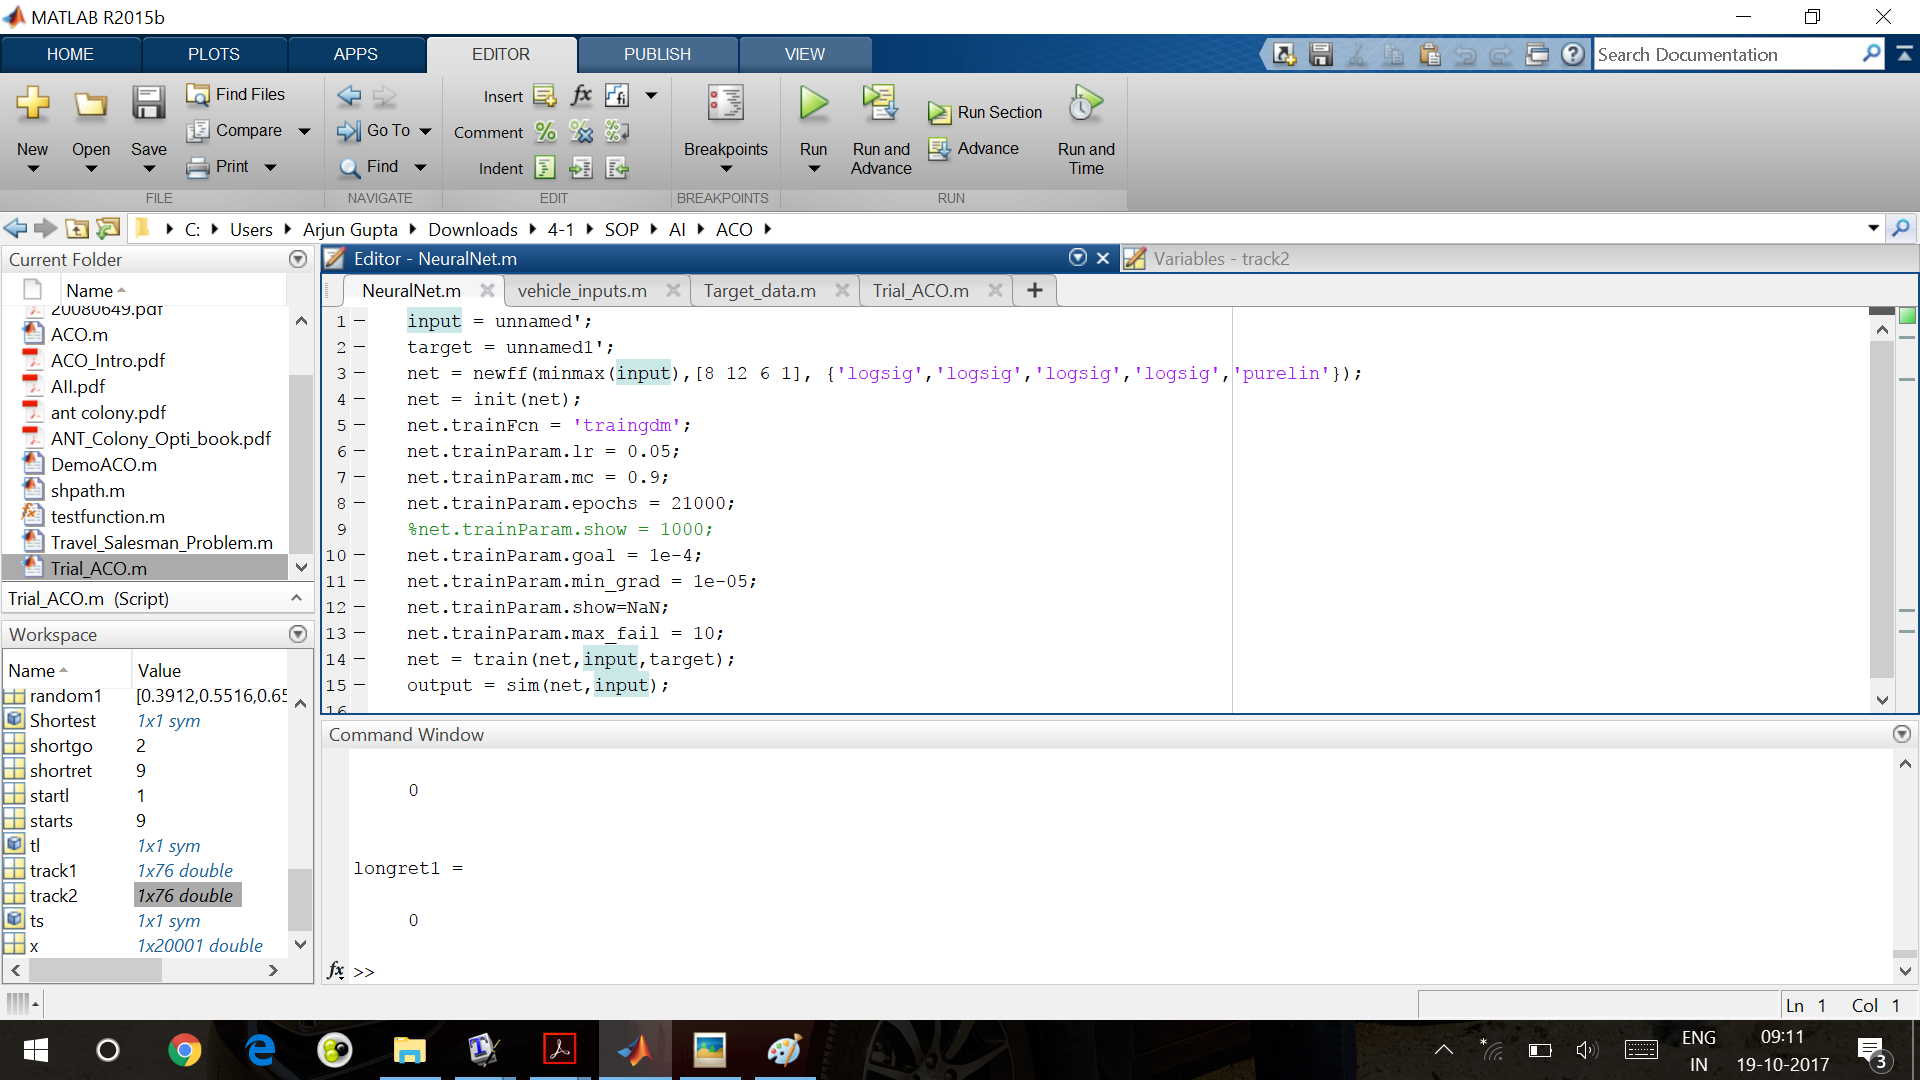
\includegraphics[height =3 in, width = \linewidth]{Neural_Net_code.png}
\caption{Parameters for Neural Network}
\label{fig3} 
\end{figure}

\begin{figure}[!h]
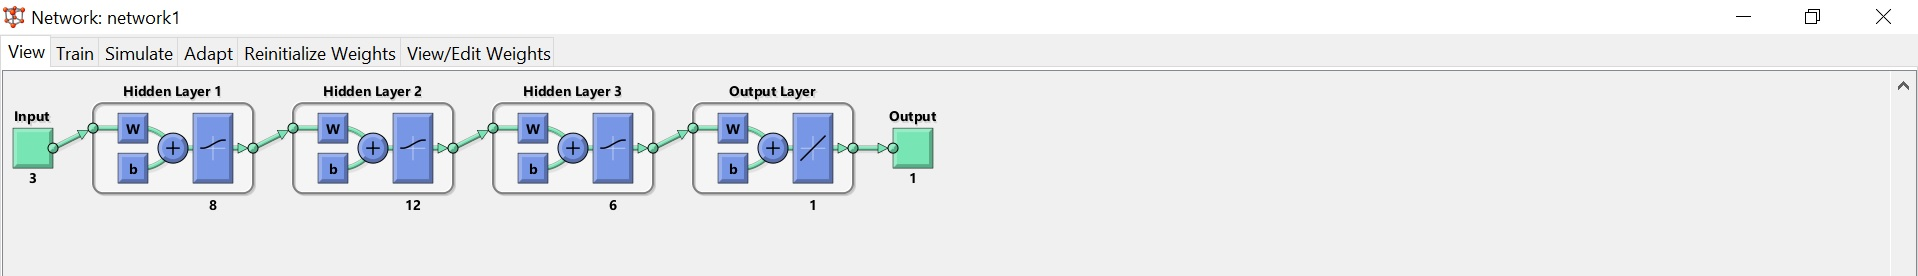
\includegraphics[height =2 in, width = \linewidth]{Layer_Struct}
\caption{Neural Network for the model}
\label{fig4}
\end{figure}

\begin{figure}[!h]
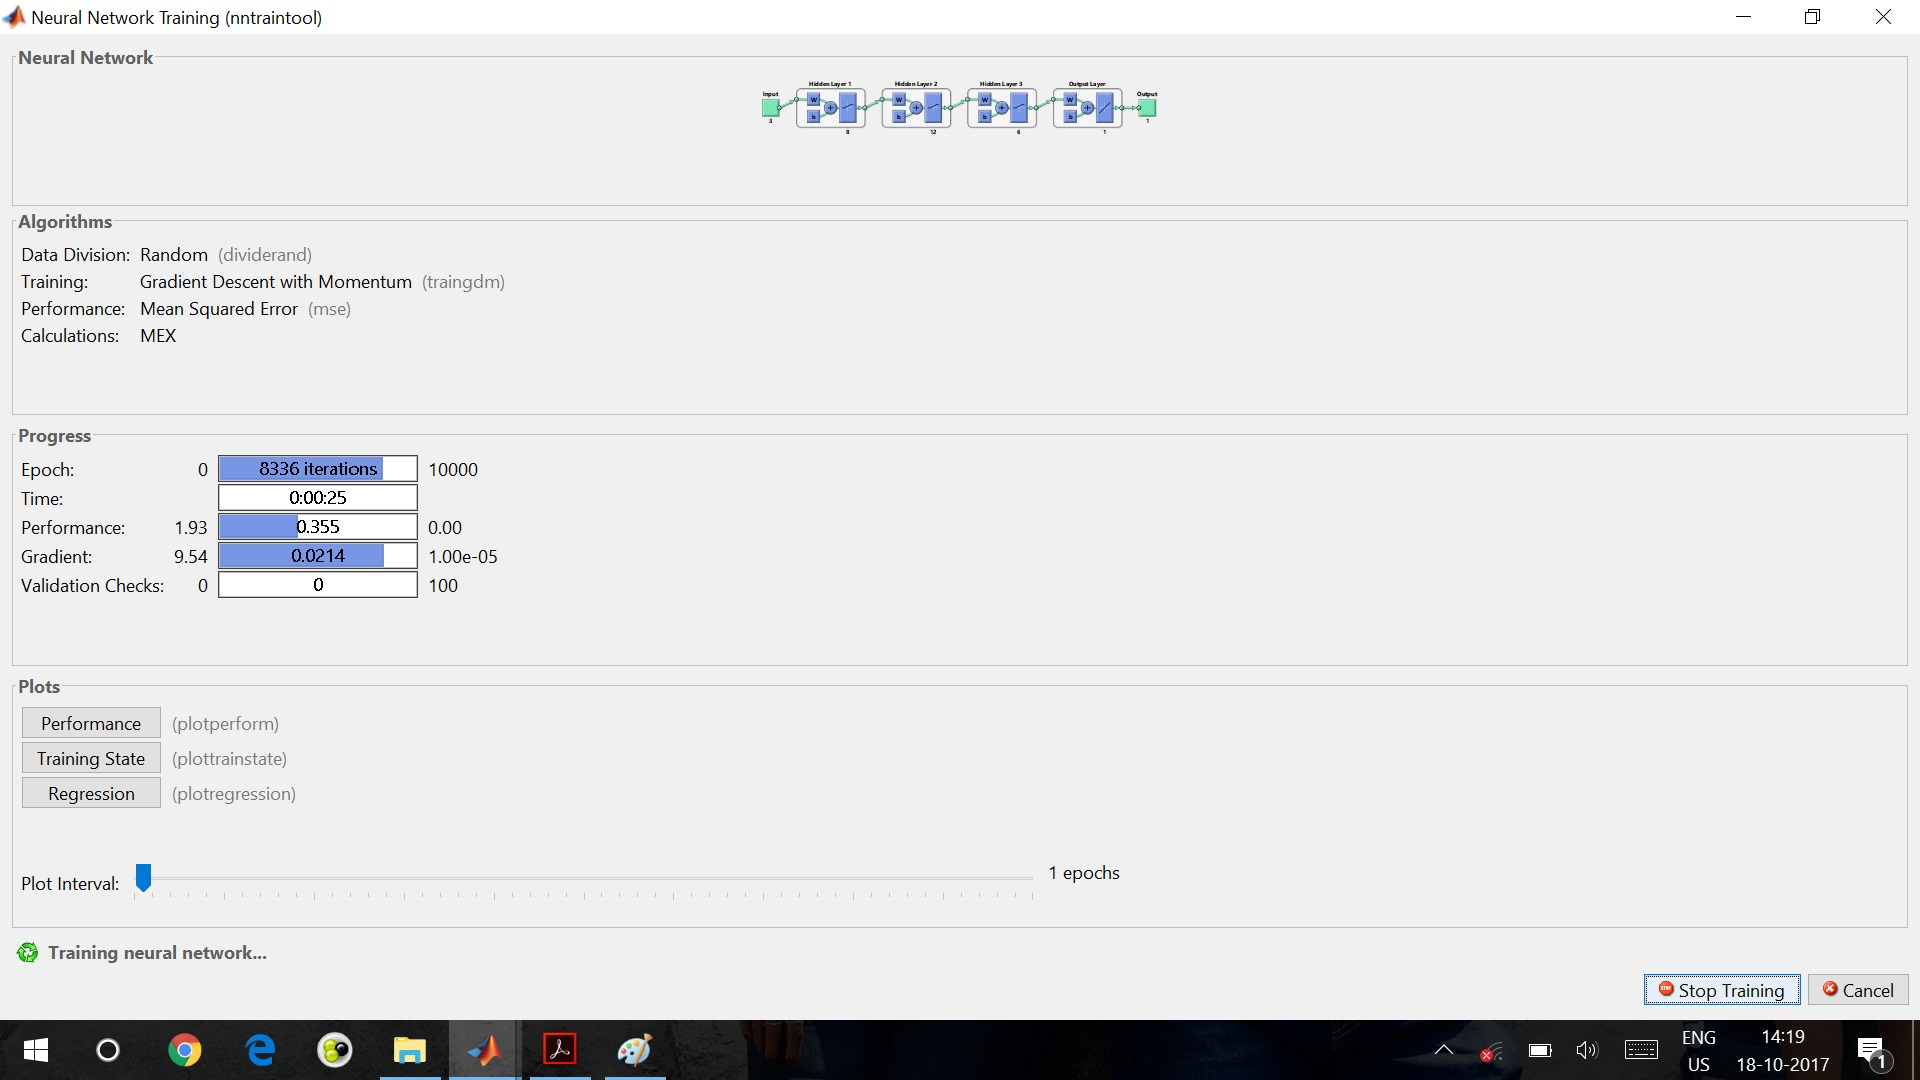
\includegraphics[height =3 in, width = \linewidth]{Neural_Train.png}
\caption{Neural Network Training Interim}
\label{fig5}
\end{figure}
\begin{figure}[!h]
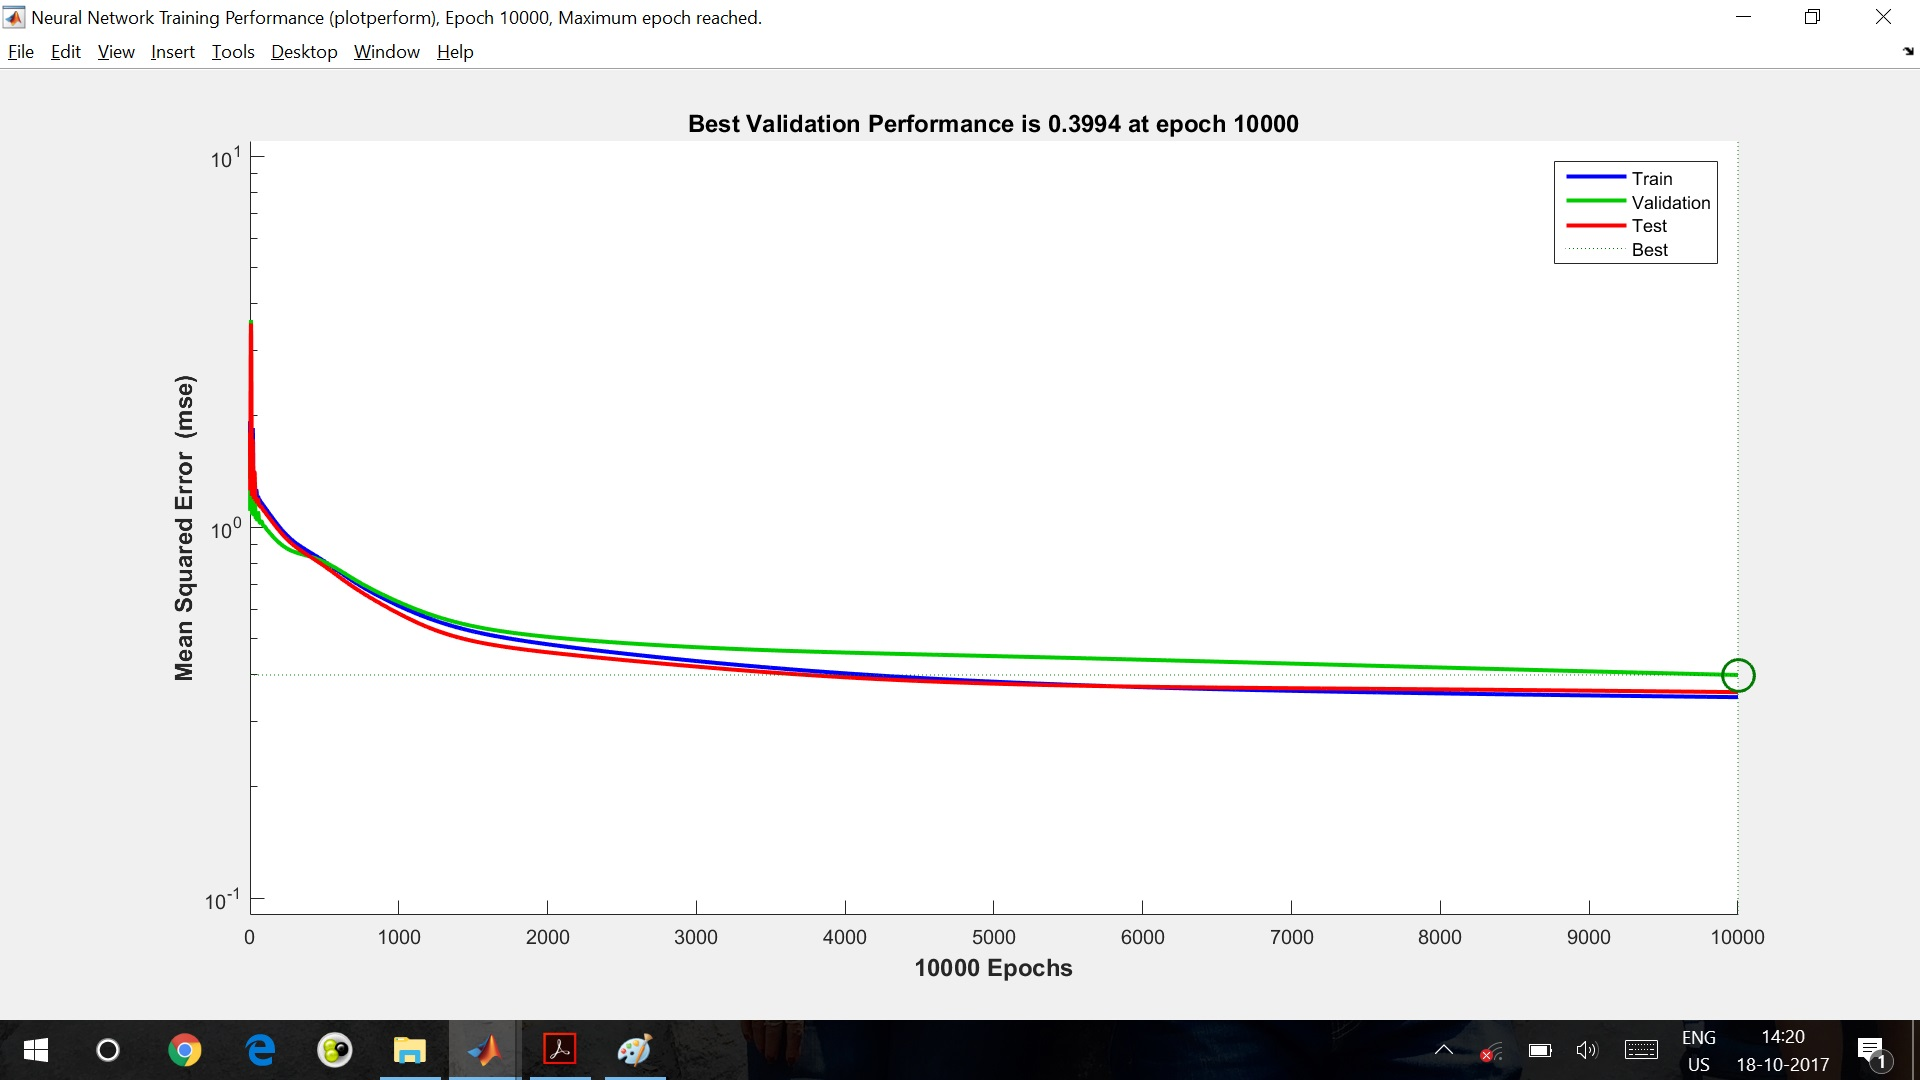
\includegraphics[height =3 in, width = \linewidth]{Performance_Graph.png}
\caption{Training Results}
\label{fig6}
\end{figure} 
\begin{figure}[!h]
\includegraphics[height =3 in, width = \linewidth]{Trajectory.png}
\caption{Trajectory as traced by the bot}
\label{fig7}
\end{figure}
\newpage

\section{Conclusion}
Robot navigation is governed and managed by a neural network working on the data obtained. We have learned about the neural networks and used back propagation algorithm to train the network. Number of layers in the network are 4. The output of our neural network gives the heading angle to the bot. Due to noise in the data obtained from the sensors the bot movement not as expected at very few instances. 
In the post mid semester duration we aim to obtain data by ourselves on a well defined path and then display the results. We also aim to implement a dynamic path planning algorithm to obtain a collision free globally optimized path and then model our controller in such a way that the bot moves towards the final point along the shortest collision free path efficiently.


\end{document}